\documentclass[11pt]{article}
\usepackage[margin=0.7in]{geometry}
\usepackage{amsmath,amssymb}
\usepackage{enumitem}
\usepackage{tikz}
\usepackage{pgfplots}
\pgfplotsset{compat=1.18}
\usepackage{fancyhdr}
\usepackage{parskip}
\setlist[enumerate]{leftmargin=*, itemsep=6pt}
\pagestyle{fancy}
\fancyhf{}
\fancyfoot[L]{\small\textit{en}Vision\textsuperscript{\textregistered} Algebra 2}
\fancyfoot[C]{\small 3-5 Lesson Quiz, short form}
\fancyfoot[R]{\small\thepage}
\renewcommand{\headrulewidth}{0pt}
\newcommand{\choice}[1]{\tikz[baseline=-0.6ex]\node[draw, circle, inner sep=0.6pt, minimum size=3.3mm, font=\scriptsize\bfseries] {#1};\;}
\newcommand{\checkbox}{$\square$\;}
\pgfplotsset{quizgrid/.style={
  axis lines=middle, grid=both, grid style={gray!45},
  ticklabel style={font=\scriptsize, fill=white, inner sep=1pt},
  xlabel={$x$}, ylabel={$y$}, axis line style={thick}, clip=true}}

\begin{document}

\noindent\textbf{Name}\; \rule{6cm}{0.4pt} \hfill Period \rule{1.2cm}{0.4pt} \quad Date \rule{2.2cm}{0.4pt}

\vspace{4pt}\noindent\rule{\textwidth}{0.6pt}

\vspace{2pt}\noindent{\LARGE\textbf{3-5 \; Lesson Quiz: Zeros of Polynomial Functions}} \hfill {\small short form}

\vspace{4pt}\noindent\rule{\textwidth}{0.6pt}

\begin{minipage}[t]{0.52\textwidth}
\textbf{1.} \textbf{Part A} What are all the zeros of $f(x)=x^3+2x^2-3x$?

Show your factoring:

\vspace{12pt}\rule{\linewidth}{0.4pt}

\vspace{12pt}\rule{\linewidth}{0.4pt}

\vspace{6pt}
Zeros: \rule{4.5cm}{0.4pt}

\vspace{6pt}
\textbf{Part B} Use the zeros to sketch the graph of $f$.
\end{minipage}\hfill
\begin{minipage}[t]{0.45\textwidth}
\vspace{-6pt}
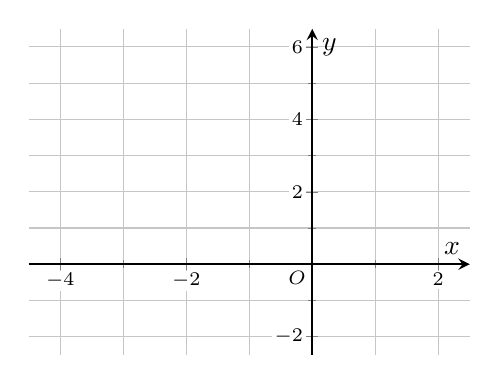
\begin{tikzpicture}
% TE window: x labels -4,-2,O,2; y labels 6,4,2,-2; grid at every unit.
\begin{axis}[quizgrid, xmin=-4.5, xmax=2.5, ymin=-2.5, ymax=6.5,
  xtick={-4,-2,2}, ytick={-2,2,4,6}, minor xtick={-4,...,2}, minor ytick={-2,...,6}, x=0.8cm, y=0.46cm]
\node[font=\scriptsize, fill=white, inner sep=1pt, anchor=north east] at (axis cs:-0.05,-0.1) {$O$};
\end{axis}
\end{tikzpicture}
\end{minipage}

\vspace{4pt}\noindent\rule{\textwidth}{0.4pt}

\begin{minipage}[t]{0.52\textwidth}
\textbf{4.} What are the zeros and their multiplicities for the function $y=x^3+3x^2+x+3$, shown in the graph?

\vspace{4pt}
\begin{itemize}[leftmargin=1.2em, itemsep=3pt, topsep=2pt]
\item[] \choice{A} $-3$, $-1$, and $1$, each multiplicity 1
\item[] \choice{B} $-3$, multiplicity 1
\item[] \choice{C} $3$, multiplicity 2
\item[] \choice{D} $-3$, multiplicity 3
\end{itemize}

How does the graph (or the equation) tell you? \par
\vspace{10pt}\rule{\linewidth}{0.4pt}
\end{minipage}\hfill
\begin{minipage}[t]{0.45\textwidth}
\vspace{-6pt}
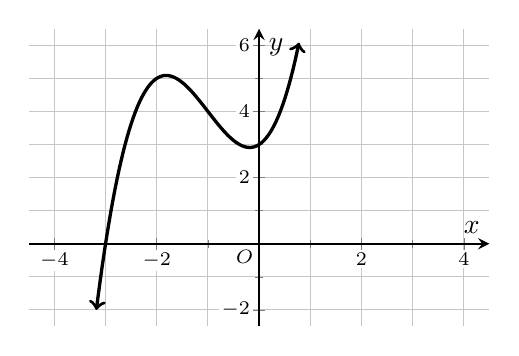
\begin{tikzpicture}
% TE window: x labels -4,-2,O,2,4; y labels 6,4,2,-2; grid at every unit; both ends inside the window so both arrowheads show.
\begin{axis}[quizgrid, xmin=-4.5, xmax=4.5, ymin=-2.5, ymax=6.5,
  xtick={-4,-2,2,4}, ytick={-2,2,4,6}, minor xtick={-4,...,4}, minor ytick={-2,...,6}, x=0.65cm, y=0.42cm]
\addplot[very thick, domain=-3.18:0.78, samples=100, <->] {x^3+3*x^2+x+3};
\node[font=\scriptsize, fill=white, inner sep=1pt, anchor=north east] at (axis cs:-0.05,-0.1) {$O$};
\end{axis}
\end{tikzpicture}
\end{minipage}

\vspace{4pt}\noindent\rule{\textwidth}{0.4pt}

\textbf{5.} Find the zeros of $f(x)=-x^3-2x^2+7x-4$. Then describe the behavior of the graph of $f$ at each zero.

\vspace{2pt}
\begin{itemize}[leftmargin=1.2em, itemsep=2pt, topsep=2pt]
\item[] \choice{A} $4$, $-1$; As $x\to-\infty$, $f\to-\infty$. When $-1<x<4$, $f<0$. At $x=4$, $f$ is tangent to the $x$-axis, so when $x>1$, $f\to\infty$.
\item[] \choice{B} $-4$, $1$; As $x\to-\infty$, $f\to-\infty$. When $-4<x<1$, $f>0$. At $x=1$, $f$ is tangent to the $x$-axis, so when $x>1$, $f\to-\infty$.
\item[] \choice{C} $4$, $-1$; As $x\to-\infty$, $f\to\infty$. When $-1<x<4$, $f>0$. At $x=4$, $f$ is tangent to the $x$-axis, so when $x>1$, $f\to-\infty$.
\item[] \choice{D} $-4$, $1$; As $x\to-\infty$, $f\to\infty$. When $-4<x<1$, $f<0$. At $x=1$, $f$ is tangent to the $x$-axis, so when $x>1$, $f\to-\infty$.
\end{itemize}

Show your work (test a zero, divide, factor):

\vspace{12pt}\rule{\textwidth}{0.4pt}

\vspace{10pt}\rule{\textwidth}{0.4pt}

\vspace{2pt}
\noindent\textbf{Scoring:} Question 1 (Parts A and B together) and Question 5 are 10 points each. Question 4 is a bonus of up to 5 points. Total out of 20. {\small (Numbers match the Savvas Lesson Quiz; Questions 2 and 3 are not on this form.)}

\newpage
\noindent{\LARGE\textbf{3-5 Lesson Quiz, short form: answer key}}

\vspace{4pt}\noindent\rule{\textwidth}{0.6pt}

\begin{enumerate}
\item \textbf{Part A: $-3$, $0$, $1$.} $f(x)=x(x^2+2x-3)=x(x+3)(x-1)$. Savvas item 1A, DOK 2, Realize skill F62. \textbf{Part B:} a cubic rising to the right that crosses the $x$-axis at $-3$, $0$ and $1$: below the axis for $x<-3$, above on $-3<x<0$ (local maximum near $(-1.9,\,6.1)$), below on $0<x<1$ (local minimum near $(0.5,\,-0.9)$), above for $x>1$. Savvas item 1B, DOK 2, Realize skill A73. Taught by Example 1 and Try It 1a. \textbf{10 points:} Part A 4 (2 for the factored form, 2 for all three zeros); Part B 6 (2 for crossing at the three zeros, 2 for the correct side of the axis on each interval, 2 for the end behavior).
\item[4.] \textbf{B, $-3$, multiplicity 1.} By grouping, $x^3+3x^2+x+3=x^2(x+3)+(x+3)=(x+3)(x^2+1)$. The factor $x+3$ appears once, and the graph crosses at $-3$ with no flattening; $x^2+1$ gives $\pm i$, which are not $x$-intercepts. Distractor A invents $\pm1$; D would flatten at $-3$. Savvas item 4, DOK 1, Realize skill F62. Taught by Example 2 (multiplicity) with factoring by grouping. \textbf{Bonus 5:} B with a reason (the factored form, or ``crosses once without flattening''); 3 for B alone.
\item[5.] \textbf{D.} $f(1)=-1-2+7-4=0$; synthetic division by $1$ gives $-x^2-3x+4$, so $f(x)=-(x-1)(x^2+3x-4)=-(x-1)^2(x+4)$. Zeros $-4$ (multiplicity 1, crosses) and $1$ (multiplicity 2, tangent). The leading term $-x^3$ gives $f\to\infty$ as $x\to-\infty$ and $f\to-\infty$ as $x\to\infty$; $f(0)=-4<0$, so $f<0$ on $-4<x<1$. Savvas item 5, DOK 2, Realize skill F62. Taught by Examples 1 and 2; rehearsed by the packet Practice. \textbf{10 points:} 6 for D, 4 for the work (a zero tested and the factored form, or $f(1)=0$ and $f(-4)=0$ checked).
\end{enumerate}

\textbf{Items left off this form} (available for a retake or Form B): Savvas item 2, solve $x^3+5x^2-x-7=x^2+6x+3$ (answer $x=-5$, $x=-1$, $x=2$; DOK 2, F62; Example 5, cut); Savvas item 3, solve $x^3-4x>0$ (answer $-2<x<0$ or $x>2$, the union of the two intervals; the TE prints ``and''; DOK 2, F62; Example 6, cut).

\textbf{Graphs:} the Question 4 graph is redrawn from the TE description and the function itself (crosses at $-3$, turning points near $(-1.8,\,5.1)$ and $(-0.2,\,2.9)$, $y$-intercept 3). The Question 1 Part B answer graph is not printed; students sketch on a blank grid.

\textbf{IXL replacement:} SmartScore 70 or above on PVM, 8CQ and NCY replaces this quiz with 20/20.

\end{document}
